
\begin{figure}[!htbp]
    \begin{centering}
        \subfloat[Maximum resident set size when correcting 50kb matrix]
        {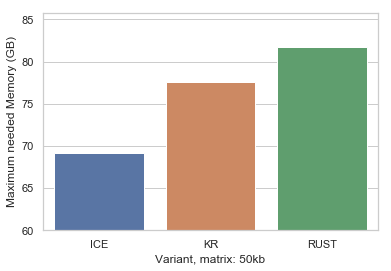
\includegraphics[scale=0.9]{figures/results/maxresident_50}} \\
        % \caption[Maximum needed Memory for 50kb]
        % {\textbf{Maximum needed Memory} when correcting the 50kb matrix.}
        \subfloat[Maximum resident set size when correcting 25kb matrix]
        {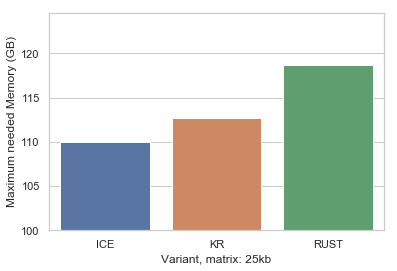
\includegraphics[scale=0.9]{figures/results/maxresident_25}}
        \caption[Maximum needed Memory]
        {\textbf{Maximum amount of needed Memory} when correcting 50kb and 25kb
        matrix. Smaller is better.}
        \label{fig:maxresident}
    \end{centering}
\end{figure}


